
\section{The  two-fluid model}
\label{sec:conservation_laws}

In this section we define the local scale governing equations of multiphase flow using the formulation of \citet{kataoka1986local} and \citet{drew1983mathematical}.
Before diving into the derivation we would like to emphasize that the local position vector at the local scale is noted $\textbf{y}$.
This clarification will have its usage in the next section where we will use another variable for the global location, namely the vector $\textbf{x}$.
Also, in this manuscript we write in bold symbols the vectors and tensors, while the scalar variables are written with the usual font.



\subsection{Evolution of the topology}

Before introducing the physical balance equations such as the mass and momentum conservation equations, we study the transport of the volume occupied by a phase $k$ and the interface between the phases considered.
Therefore, the topological balance equations correspond to the transport equations of $\chi_k$, and the transport of its \textit{roots} along the velocity of its interfaces.

\begin{figure}[h!]
    \centering
    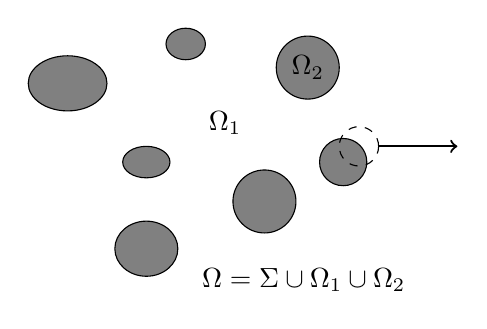
\begin{tikzpicture}
        \foreach \x/\y/\ra/\r in {
        1/3/0.2/0.25,
        2.55/2.7/0.4/0.4,
        0.5/0.4/0.35/0.4,
        2/1/0.4/0.4,
        3/1.5/0.3/0.3,
        0.5/1.5/0.2/0.3,
        -0.5/2.5/0.35/0.5}{
            \draw[fill=gray](\x,\y) ellipse(\r cm and \ra cm);
        }
        \draw[dashed](3.2,1.7)circle(0.25);
        % \draw[thick,->](3.2,1.7)++(0.1767,0.1767)--++(0.4,0.4)--++(1,0);
        \draw[thick,->](3.2,1.7)++(0.25,0)--++(1,0);
        \draw(2.55,2.7)node{$\Omega_2$};
        \draw(1.5,2)node{$\Omega_1$};
        \draw(2.5,0)node{$\Omega = \Sigma \cup \Omega_1 \cup \Omega_2$};
        % \draw(2.5,-1)node{$\Sigma = \sum_\alpha \Sigma_\alpha$};
        % \draw(2.5,-0.5)node{$\Omega_2 = \sum_\alpha \Omega_\alpha$};
    \end{tikzpicture}
    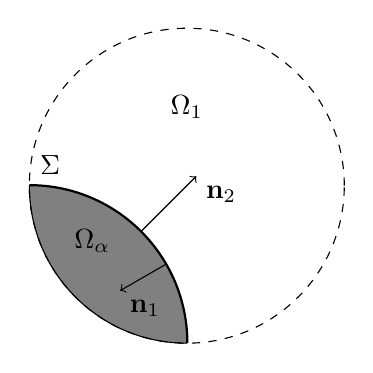
\begin{tikzpicture}%[scale = 0.9]
        \draw[very thick](0:2)arc(0:90:2)node[above right]{$\Sigma$};
        \draw[fill=gray](0:2)arc(0:90:2)arc(180:270:2);
        \draw[dashed](2,2)circle(2);
        \draw[->](1.42,1.42)--++(0.7,0.7)node[below right]{$\textbf{n}_2$};
        \draw[->](1.73,1)--++(-0.577,-0.333)node[below right]{$\textbf{n}_1$};
        \draw(2,3)node{$\Omega_1$};
        \draw(0.8,1.3)node{$\Omega_\alpha$};
    \end{tikzpicture}
    \caption{Scheme of the topology of dispersed two phase flows.}
\end{figure}
To carry out the derivation of these equations we first introduce the Phase Indicator Function (PIF),
\begin{equation}
    \chi_k(\textbf{y}) =  \left\{
      \begin{tabular}{cc}
        $1 \;\text{if} \;\textbf{y} \in \Omega_k$\\
        $0 \;\text{if} \;\textbf{y} \notin \Omega_k$
      \end{tabular}
      \right.,
      \label{eq:phase_indicator}
\end{equation}
with $V_k$ the volume occupied by the $k^{th}$ phase.
As an example, $V_c$ is the volume occupied by the continuous phase and $V_d$ by the dispersed phase.
With the use of this function we will be able to generalize the phase quantities to general fields, and to derive two kinds of conservation equations, namely, the single-fluid formulation and the two-fluid formulation.

First, the transport equation of $\chi_k$ reads as \citep{drew1983mathematical,kataoka1986local,morel2015mathematical},
\begin{equation}
    \pddt \chi_k
    + \textbf{u}_I \cdot \nablabh \chi_k
    = 0,
    \label{eq:phaseindicator_transport}
\end{equation}
where $\textbf{u}_I$ is the velocity of the interface.
It is important here to make the distinction between the velocity \textbf{of the interface} which is different from the velocity of the phase $k$ \textbf{at the interface} location which is noted $\textbf{u}_k$.
Besides, it can be shown \citep{tryggvason2011direct} that,
\begin{equation}
    \nablabh \chi_k
    = - \delta_I \textbf{n}_k
\end{equation}
where we have introduced the interface indicator function $\delta_I$, defined as $\delta(\textbf{y}-\textbf{y}_I)$, where $\delta$ is the Dirac-delta function and $\textbf{y}_I$ the position vector of the interfaces.
We also define $\textbf{n}_k$ as the outward normal vector of the phase $k$.

As pointed out by \citet{morel2007surface}, this equation can be rewritten under the more common form,
\begin{equation}
    \pddt \delta_I
    + \nablabh \cdot (\delta_I \textbf{u}_I)
    = \delta_I \nablabhI \cdot \textbf{u}_I.
    \label{eq:interface_transport2}
\end{equation}
Notice that now the velocity involved is simply $\textbf{u}_I$ and not the normal velocity $\textbf{u} \cdot \textbf{n}$ as in \ref{eq:interface_transport}.
Also, it can be useful to derive an expression for the gradient of the $\delta_I$ function. 
To do so we take the gradient of \ref{ap:eq:phase_properties} yielding, 
\begin{align*}
    &\nablabh\delta_I 
    = \textbf{n} \cdot \nablabh (\textbf{n} \delta_I),
    &
    \pddt\delta_I 
    = - \textbf{n} \cdot \nablabh (\textbf{u}_I  \cdot \textbf{n} \delta_I)
\end{align*}


\subsection{Local conservation equations}
Any conservation equation for an arbitrary quantity $f_k(\textbf{y})$, where $f_k$ represent the quantity $f$ but defined in the arbitrary phase $k$, will takes the form,
\begin{align}
    \label{eq:general_conservation}
    \pddt f_k
    &= \nablabh \cdot \left(
        \bm{\Phi}_k
        - f_k\textbf{u}_k
        \right)
    + \textbf{S}_k
    & \forall \textbf{y} \in \Omega_k&\\
    \pddt f_I  
    &= 
    \nablabhI \cdot (\mathbf{\Phi}_{||}^I - f_I \textbf{u}_I)
    + \textbf{S}_I
    - \Jump{
        f_k (\textbf{u}_I - \textbf{u}_k)
        + \mathbf{\Phi}_k
     } 
    & \forall \textbf{y} \in \Sigma&
    \label{eq:dt_f_I}
\end{align}
where $\nablabh\cdot()$ is the local divergence operator defined as, $\frac{\partial}{\partial \textbf{y}}\cdot()$, $\textbf{u}_k$ is the phase velocity defined in the phase $k$.
$\bm{\Phi}_k$ is the non-conservative flux corresponding to the quantity $f_k$,
The non-conservative flux is often expressed through a constitutive equation depending on the nature of the flow such as the stress tensor for the momentum.
And $\textbf{S}_k$ is the volumetric source of $f_k$, such as the body forces still for the momentum equation.
It is important to notice that \ref{eq:general_conservation} is solely defined in the volume occupied by the phase $k$.
To generalize the conservation equation over the whole domain, i.e. in each phase and also at the interfaces, we will need supplementary equations.


\subsection{Global conservation equations}

As stipulated above, \ref{eq:general_conservation} is solely defined on phase $k$.
We thus need to generalize this equation over the whole domain constituted by all phases.
There are two possible formulations to carry out this task.
In the following, we give a brief overview of both formulations in the case of a general conservation equation such as \ref{eq:general_conservation}.
The first formulation is the so-called \textit{Two-fluid formulation}.
In this formulation we transport the quantity $f_k\chi_k$, so that $f_k\chi_k$ is defined over the whole domain, since $\chi_k f_k = f_k$ where $\textbf{y} \in V_k$ and $\chi_k f_k = 0$ else where.
So we derive the so called \textit{two-fluid} formulation by multiplying \ref{eq:general_conservation} by the PIF, $\chi_k$ and rearranging each term.
By making use of the \ref{eq:phaseindicator_transport}, it yields
\begin{align}
    \pddt (\chi_k f_k)
    &= \nablabh \cdot (\chi_k \bm{\Phi}_k - \chi_k f_k \textbf{u}_k)
    + \chi_k \textbf{S}_k
    + \delta_I\left[
        \bm{\Phi}_k
        + f_k
        \left(
            \textbf{u}_I
            - \textbf{u}_k
        \right)
    \right]
    \cdot \textbf{n}_k ,
    % & \forall \textbf{y} \in \Omega&
    \label{eq:two-fluid_global}\\
    \pddt (\delta_If_I)  
    &= 
    \nablabh \cdot (\delta_I \mathbf{\Phi}_{I||} - \delta_I f_I \textbf{u}_I)
    +\delta_I\textbf{S}_I 
    - \delta_I \Jump{
    f_k (\textbf{u}_I - \textbf{u}_k)
    + \mathbf{\Phi}_k
    } 
    \label{ap:eq:general_jump}
\end{align}
where the last term is the interfacial source term representing the interactions across the phases.
As an example, if $f_k$ turns out to be the momentum, then the interfacial source term would be the drag forces between the phases (see next section).
As desired, in this equation all quantities $f_k$ are factor of $\chi_k$.
So we transport the field $\chi_k f_k$, which is a field quantity defined over the whole domain.
Notice that the interfacial term is factor of $\delta_I$ instead of $\chi_k$ as it is defined on the interface.
Anyhow, \ref{eq:two-fluid_global} is defined over the entire domain and is therefore considered as a valid transport equation.

Now that we properly defined any conservation laws inside and across each phase, let's derive the \textit{single-fluid} formulation for \ref{eq:general_conservation}.
To do so we sum on all phases \ref{eq:two-fluid_global}, and make use of the jump condition \ref{eq:general_jump} to simplify the interfacial terms.
Besides, we define the arbitrary quantity $f$ being $f = \sum_k \chi_k f_k + \delta_I f_I$.
By taking into account these remarks it is trivial to show that,
\begin{equation}
    \pddt f
    = \nablabh \cdot (\bm{\Phi} - f \textbf{u})
    + \textbf{S}
    \label{eq:single-fluid_global}
\end{equation}
which is the \textit{single-fluid} formulation.
In the following we expose the most important conservation equations for our purpose by replacing $f_k$ or $f$ by the desired quantities.

